% Official ACL template (uses acl.sty + acl_natbib.bst in this dir / Overleaf project).
% Switch [final] -> [review] for anonymous submission (adds line numbers, hides authors).
\documentclass[11pt]{article}
\usepackage[final]{acl}
\usepackage{times}
\usepackage{latexsym}
\usepackage[T1]{fontenc}
\usepackage[utf8]{inputenc}
\usepackage{microtype}
\usepackage{booktabs}
\usepackage{graphicx}
\usepackage{amsmath}
\usepackage{amssymb}
\usepackage{xcolor}
\usepackage{multirow}

\newcommand{\ona}{\textsc{ona\_tili}}
\newcommand{\tarix}{\textsc{tarix}}
\newcommand{\bsfs}{\textsc{BootstrapFewShot}}

\title{Anatomy and Repair of a Native-Language ``Erosion'':\\
Prompt Optimization and Token Budgets}

\author{
  Dovud Asadov\textsuperscript{1,2} \quad
  Abduaziz Kayumov\textsuperscript{2} \quad
  Qobiljon Toshnazarov\textsuperscript{2} \\
  Mardonbek Hazratov\textsuperscript{1,2} \quad
  Husanboy Mansuraliyev\textsuperscript{1,2} \\[2pt]
  \textsuperscript{1}IDROCK AI Excellence Center, New Uzbekistan University \\
  \textsuperscript{2}New Uzbekistan University \\
  \texttt{\{d.asadov,\,a.kayumov,\,q.toshnazarov\}@newuu.uz}
}

\begin{document}
\maketitle

\begin{abstract}
Automatic prompt optimizers such as \textsc{DSPy}'s \bsfs{} are marketed as turnkey
accuracy boosters and increasingly applied to low-resource languages. In earlier work
we reported that \bsfs{} erodes the native-language subject (\ona{}, Uzbek grammar and
literature) of a subject-partitioned university-entrance benchmark while aggregate
accuracy stays flat (pooled McNemar $p{=}0.011$), and that the intuitive
mechanism---demonstration subject-skew---is not the cause. This paper identifies what
causes it, corrects two of our own claims, and repairs one route to the harm---while
showing a second route remains. With a fully instrumented harness (raw completions,
token usage, finish reasons) we show:
(1) one route to the ``erosion'' is a \emph{deployment-regime artifact}: correctness-based selection
sometimes imports verbose reasoning-subject demonstrations that violate the prompt's
own brevity instruction, inflate responses into a fixed decoding budget, and surface as
truncation and parse failures concentrated on the subject with the longest inputs.
Excluding those failures, our original headline weakens to $p{=}0.073$.
(2) the budget lever is \emph{causal}: raising \texttt{max\_tokens} from 256 to 2048
removes truncations monotonically (Cochran--Armitage trend $p{<}10^{-4}$).
(3) at scale the native language is \emph{not} intrinsically fragile: a powered
within-subject test ($n{=}3{,}822$ paired items, six models, two test sets) finds no
knowledge-side erosion---overturning our earlier single-model full-precision result.
(4) the effect's sign flips across serving stacks \emph{and} between 4-bit and
16-bit precision in all three large models, because numerics change which demonstrations the optimizer
self-selects.
(5) a one-line \emph{constraint-consistent} bootstrapping metric plus rescue parsing
recovers $85.6\%$ of the erosion while retaining $108\%$ of the math gains, passing a
pre-registered bar.
(6) on a second language (\textsc{TurkishMMLU}, six models) the concealment is starker
while the mechanism does not travel: aggregate accuracy rises $5.2$ points as the
native subject gains nothing, and conditional on an item changing answer, native items
change for the worse at $2.35\times$ the odds of non-native ones ($95\%$ CI
$[1.38, 4.17]$, bootstrapping over items), closely matching the $2.27$ we obtain on our
original stack---yet the absolute native drop is null ($p{=}1.0$) and $35$ of $37$
Turkish native losses are well-formed, in-budget answers that our repair cannot touch. A second, content-side
route to the same harm therefore exists, and we do not explain it. Finally,
(7) the differential is \emph{not} a \bsfs{} artifact: \textsc{MIPROv2}, which searches
instructions rather than selecting correct demonstrations, reproduces it at the same
magnitude on the same stack ($1.75$ vs.\ $1.63$). It also confirms the mechanism from
the opposite side---its \emph{more} verbose demonstrations produce a quarter of the
format failures, because the instruction it writes enforces the format they violate,
which implies a second repair. We release the instrumented harness, per-item logs for
every number, and a frozen replication set.
\end{abstract}

\section{Introduction}
Chain-of-thought (CoT) prompting of large language models (LLMs)~\citep{wei2022cot}
helps mainly on math and symbolic reasoning~\citep{sprague2025cot} and can hurt
elsewhere~\citep{liu2025mind}. On top of
CoT, automatic prompt optimizers---most prominently
\textsc{DSPy}~\citep{khattab2024dspy} with its \bsfs{} teleprompter, which retains as
few-shot demonstrations only training examples the model itself answers
correctly---are increasingly applied to low-resource languages, where the subject a
model is weakest at is typically the users' own language.

In earlier work we reported a small but statistically significant cost hidden by the
aggregate metric. On \textbf{DTM}~\citep{dtm2026}, a subject-partitioned Uzbek
university-entrance benchmark built from materials of the national State Test Center
(\emph{Davlat Test Markazi}, DTM), \bsfs{} left overall accuracy roughly flat while
eroding \ona{} (Uzbek grammar and literature) in five of six open LLMs (pooled McNemar
$p{=}0.011$, mean $-4.8$), and a controlled experiment ruled out the intuitive
mechanism, demonstration subject-skew. We closed by conceding the true mechanism was
unknown.

This paper answers that open question---and in doing so corrects our own record. We
re-instrumented the entire pipeline to log raw completions, token usage, and finish
reasons for every generation, then subjected the finding to a causal budget
manipulation, a demonstration-length manipulation, a powered within-subject test with
a frozen replication set, a fixes shoot-out with a pre-registered success bar, and
full-precision (16-bit brain floating point, bf16) coverage of the large models. Our contributions:

\begin{itemize}\itemsep1pt
\item \textbf{A mechanism} (\S\ref{sec:fragility}--\S\ref{sec:budget}).
Correctness-selection imports verbose reasoning-subject demonstrations that contradict
the prompt's own brevity instruction, and under a fixed budget the inflated responses
truncate and fail to parse on the subject with the longest inputs. Roughly a third of
our original pooled flips were such failures (clean-item $p{=}0.073$). The lever is
causal: truncations fall $28{\to}16{\to}3{\to}0$ across budgets $256{\to}2048$ (trend
$p{<}10^{-4}$), against a flat zero-truncation control.
\item \textbf{Two corrections} (\S\ref{sec:fragility}, \S\ref{sec:powered}). The
observational effect does not replicate across serving stacks ($p{=}0.227$), because
different numerics select different demonstrations. And our earlier ``robustness''
result ($-7.2$, $p{=}0.045$, $n{=}250$, one model) is overturned by a powered version
($n{=}3{,}822$ paired items, six models): no knowledge-side erosion.
\item \textbf{Negative controls} (\S\ref{sec:demos}). Demonstration \emph{subject} is
null, and \emph{length} is null in the mild-payload regime---the harm needs the
extreme-payload $\times$ tight-budget corner. Models rarely write long native-language
reasoning at all, so the budget-breaking register is an import from reasoning subjects.
\item \textbf{A repair} (\S\ref{sec:fixes}). Requiring bootstrapped demonstrations to
satisfy the prompt's own brevity constraint, plus rescue parsing, recovers $85.6\%$ of
the erosion while retaining $108\%$ of the math gains, passing a pre-registered bar.
\item \textbf{Instability} (\S\ref{sec:precision}). Every large model's delta flips sign
between Q4 and bf16, and our own tokenizer-fertility hypothesis is falsified by the
logs: math \emph{outputs} cost more tokens than Uzbek prose.
\item \textbf{Generalization, with an honest failure} (\S\ref{sec:travel}). On
\textsc{TurkishMMLU} aggregate accuracy rises $5.2$ points while the native subject
gains nothing, and native items change for the worse at $2.35\times$ the odds of
non-native ones ($[1.38, 4.17]$). But the absolute drop is null and our mechanism does
\emph{not} travel: $35$ of $37$ native losses are well-formed in-budget answers. The
harm generalizes. Our explanation of it does not.
\item \textbf{Not one optimizer's artifact} (\S\ref{sec:optimizer}). \textsc{MIPROv2}
reproduces the differential at the same magnitude ($1.75$ vs.\ $1.63$) and confirms the
mechanism from the opposite side: its \emph{more} verbose demonstrations produce a
quarter of the format failures, because the instruction it writes enforces the format
they violate.
\end{itemize}

The upshot inverts our earlier caution without weakening it: the native language is
not intrinsically harmed by prompt optimization, but the deployment stack can
manufacture a harm that looks exactly like it---and, as Turkish shows, at least one
further route to the same harm remains unexplained. Audits must therefore run per
subject \emph{on the deployment stack}, score parse failures separately from knowledge
errors, and constrain optimizers to respect their own prompts. We release the harness,
per-item logs behind every number, and the replication set.

\section{Related Work}\label{sec:related}
\paragraph{When CoT helps and hurts.} CoT's gains concentrate on math and symbolic
tasks~\citep{sprague2025cot}. It can reduce accuracy on tasks where deliberation hurts
humans~\citep{liu2025mind}, and its marginal value on strong models is
shrinking~\citep{meincke2025decreasing}. We study the \emph{optimizer} layered on CoT
and find its native-language cost flows through format compliance, not knowledge.
\paragraph{Automatic prompt optimization.} \textsc{DSPy}~\citep{khattab2024dspy} and
\textsc{MIPROv2}~\citep{opsahlong2024mipro} self-bootstrap demonstrations.
\citet{sarmah2024} conjectured teleprompters over-rely on examples the model already
answers well. We measured that skew previously and here show the harm it correlates
with is transmitted by demonstration \emph{payload meeting budget}, not subject.
\paragraph{Format restrictions and budgets.} Format constraints degrade reasoning
performance~\citep{tam2024format}. Tokenizers price languages
unequally~\citep{petrov2023tokenizer}, with accuracy consequences across low-resource
languages~\citep{lundin2025tokentax}. We connect this literature to prompt
optimization: the optimizer is a mechanism that \emph{generates} format pressure, and
fixed decoding budgets convert it into subject-selective failures---though, contrary
to our own initial hypothesis, through input length and induced verbosity rather than
output-side fertility (\S\ref{sec:precision}).
\paragraph{Cross-lingual reasoning dynamics.} A parallel literature asks which language
multilingual models reason \emph{in}: latent-language analyses of English-centric
internal processing~\citep{wendler2024llamas,schut2025english,zhong2024english}, how
language-centric pretraining shapes reasoning~\citep{park2025collapse}, and reasoning
transfer into extremely low-resource languages~\citep{tran2025pivoted}. We do not test
these mechanisms, and flag them because they are the most plausible home for the
content-side route our own account cannot explain (\S\ref{sec:travel}): if
correctness-selected demonstrations pull generation toward a dominant-language register,
native-language answers could degrade on their merits with no format failure at all.
Deciding that needs representation-level evidence we do not collect.
\paragraph{Disparate impact.} \citet{zhu2022rich} show semi-supervised learning can
help high-baseline subgroups at low-baseline subgroups' expense, masked by averages.
Our powered test finds the low-resource analogue is, at scale, an artifact of the
serving regime rather than a learning-dynamics inevitability.
\paragraph{Uzbek and Turkic evaluation.} Native Turkic benchmarks include
TUMLU~\citep{tumlu2025}, KazMMLU~\citep{kazmmlu2025}, and
TurkishMMLU~\citep{turkishmmlu2024}. DTM~\citep{dtm2026} provides the subject
partition our analyses require.

\section{Setup}\label{sec:setup}
\paragraph{Data.} DTM~\citep{dtm2026}: $1{,}000$ four-option questions (\ona{} $400$,
\tarix{} $300$, mathematics $150$, physics $150$). Seeded stratified split (train
$500$/dev $249$/test $251$, ${\sim}100$ \ona{} test items per model). During this
study we found eight rows of the release file with nulled answers. Two fall in the
test split and their gold labels were recovered from our published run logs, six are
excluded from train/dev. A verification gate asserts our loader reproduces the
original runs' test sequence and gold labels exactly. \textbf{Replication set:} the
DTM~2019 public corpus contributes $393$ deduplicated \ona{} items never used in any
development decision. Its protocol was frozen before first model contact.
\paragraph{Models and engines.} Six open instruction-tuned LLMs spanning
\textsc{gemma-4} (\textsc{e4b}, \textsc{31b}) and \textsc{qwen-3.5/3.6}
($4$--$27$B). The original study served the models with Ollama at 4-bit quantization
(Q4\_K\_M, hereafter Q4) on an Apple-silicon workstation. The present study replicates
that configuration on an NVIDIA DGX Spark and adds vLLM at bf16 for the three large models. Greedy decoding, \texttt{max\_tokens} $512$ unless
manipulated.
\paragraph{Conditions.} \textbf{direct} (answer only), \textbf{cot}
(brevity-constrained zero-shot CoT: ``at most two sentences''), \textbf{bootstrap}
(\bsfs{} on the CoT module, $4$ demonstrations, correctness metric), and
\textbf{bootstrap-compliant} (the fix: the metric additionally requires the
demonstration's reasoning to satisfy the brevity instruction, see \S\ref{sec:fixes}).
\paragraph{Instrumentation and scoring.} Every generation logs raw completion text,
prompt/completion token counts, finish reason, and a parse-failure flag. A rescue
parser recovers answer letters from unparseable raw text. We score two ways:
\emph{deployment} (a parse failure is a wrong answer---what a user experiences) and
\emph{knowledge} (items where either condition truncated or failed to parse are
excluded). DSPy retries a failed parse through a second adapter before erroring, so
all failure counts are lower bounds on incidents.
\paragraph{Statistics.} Paired exact binomial McNemar tests throughout, with Holm
correction within each pre-registered contrast family and Cochran--Armitage for
dose trends. All numbers regenerate from committed per-item logs.

\section{The Observation, and Its Fragility}\label{sec:fragility}

\begin{table}[t]\centering\small
\caption{Per-model \ona{} change $\Delta$ (CoT${\to}$\bsfs{}) on the original stack
(Apple silicon, Q4) and the replication stack (DGX Spark, Q4): same models, seed, and
verified split, deployment-scored. The observational effect does not transfer across
stacks.}
\label{tab:twostacks}
\setlength{\tabcolsep}{4pt}
\begin{tabular}{lrr}
\toprule
Model & orig.\ stack & repl.\ stack \\
\midrule
qwen3.5:9b   & $-9$ & $-5$ \\
gemma4:e4b   & $-8$ & $-3$ \\
qwen3.5:4b   & $-5$ & $-5$ \\
qwen3.6:27b  & $-4$ & $-4$ \\
gemma4:31b   & $-3$ & $+1$ \\
qwen3.5:27b  & $\phantom{-}0$ & $+2$ \\
\midrule
pooled McNemar & $p{=}0.011$ & $p{=}0.227$ \\
\quad clean items & $p{=}0.073$ & $p{=}0.501$ \\
\bottomrule
\end{tabular}
\end{table}

Our original headline was a pooled paired erosion of \ona{} under \bsfs{}: $75$
CoT-correct answers flipped wrong against $46$ the other way (McNemar $p{=}0.011$,
mean $-4.8$---see Table~\ref{tab:twostacks}, left column). Instrumenting the shipped traces
decomposes those flips: \textbf{nine of the 29 net flips were parse
failures}---generations the DSPy adapter could not parse, scored as wrong---and they
concentrate exactly in the two models with the largest erosions (parse errors:
qwen3.5:9b $1{\to}11$, gemma4:e4b $0{\to}10$, on $n{=}100$ each). Excluding items where
either condition failed, the pooled test weakens to $p{=}0.073$. The original claim
survives as a \emph{deployment-scored} harm (users did receive unusable outputs) but
not, at conventional thresholds, as a knowledge-scored one.

\paragraph{The comparative claim survives item clustering.} Two objections apply to the
pooled test above. It treats model$\times$item pairs as independent although the same
items recur across all six models, and it measures an \emph{absolute} fall in \ona{}
rather than the comparative claim we actually make, that the native subject is harmed
while the others gain. Estimating that contrast directly---the odds that a
\emph{changed} item changed for the worse, \ona{} relative to the other three subjects,
pooled by Mantel--Haenszel with each model as its own stratum and bounded by a bootstrap
resampling items as whole clusters---gives an odds ratio of $2.27$ on the original stack
($95\%$ CI $[1.37, 3.91]$, five of six models agreeing). The interval excludes $1$. The
comparative form of our original finding therefore holds under the item clustering its
critics would apply, even as the absolute form weakens once format failures are removed.
\S\ref{sec:travel} turns the same estimator on a second language.

\paragraph{The effect does not transfer across stacks.} We re-ran the identical
protocol---same models, quantization, seed, and a loader verified to reproduce the
original test split item-for-item---on different hardware
(Table~\ref{tab:twostacks}, right column). The pooled effect is directionally
negative but far from significant ($b{=}65$, $c{=}51$, $p{=}0.227$, clean-item
$p{=}0.501$), and the two largest original erosions shrink by roughly half. The
reason is visible in the logs: \bsfs{} selects whichever training traces the model
answers correctly, and numerics differ across stacks, so the \emph{selected
demonstrations differ}. On the replication stack, gemma4:e4b's selected payload grew
to $3{,}565$ characters (original: $3{,}080$) and its vanilla-bootstrap run produced
$62$ truncated and $56$ unparseable generations across subjects (CoT: $17$/$13$),
while models whose selected payloads stayed under ${\sim}1.7$k characters produced
essentially none. The observational effect, at $n{\approx}100$ per model, is
dominated by which demonstrations the stack happens to select.

\begin{table}[t]\centering\small
\caption{Replication-stack means over six models: the prompting ladder redistributes
accuracy. On DTM the compliant-bootstrap fix (\S\ref{sec:fixes}) beats vanilla \bsfs{}
on \emph{both} subjects, which \S\ref{sec:travel} shows does not hold on
\textsc{TurkishMMLU}.}
\label{tab:ladder}
\setlength{\tabcolsep}{5pt}
\begin{tabular}{lrr}
\toprule
Condition & \ona{} & math \\
\midrule
direct (no prompting) & 32.8 & 53.1 \\
CoT                   & 33.3 & 74.6 \\
\bsfs{} (vanilla)     & 31.0 & 78.5 \\
\bsfs{} (compliant)   & \textbf{33.0} & \textbf{80.3} \\
\bottomrule
\end{tabular}
\end{table}

\paragraph{The redistribution framing survives.} What is stable across both stacks is
the \emph{shape} of the effect (Table~\ref{tab:ladder}): each rung of the prompting
ladder buys large reasoning gains (math $+21$ from CoT, $+4$ more from the optimizer)
while the native language is flat to slightly negative---and on the original stack,
five of six models ended \emph{below the no-prompting baseline} on \ona{} after the
full stack (means $32.7{\to}29.3$) even as math gained $+34$. Aggregate accuracy
cannot see this. Figure~\ref{fig:decomp} decomposes the replication-stack flips.

\begin{figure}[t]
\centering
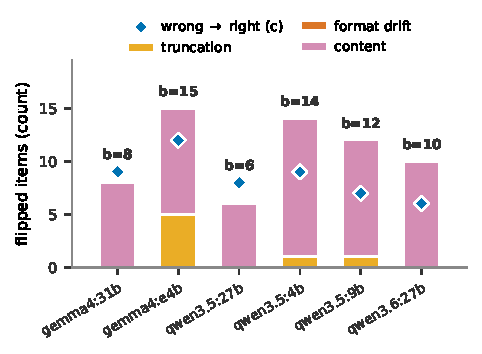
\includegraphics[width=\columnwidth]{figures/fig_decomposition.pdf}
\caption{Replication-stack decomposition of CoT-correct${\to}$bootstrap-wrong \ona{}
flips per model into truncation, format-drift, and content classes (markers: opposite
flips). Format failures concentrate where selected demonstration payloads are
largest.}
\label{fig:decomp}
\end{figure}

\section{The Budget Lever Is Causal}\label{sec:budget}

If the format component is truncation under a fixed budget, raising the budget must
remove it monotonically. It does (Table~\ref{tab:dose}). On gemma4:e4b,
bootstrap-condition truncations fall $28{\to}16{\to}3{\to}0$ as \texttt{max\_tokens}
rises $256{\to}512{\to}1024{\to}2048$ (Cochran--Armitage trend $p{<}10^{-4}$) and the
\ona{} erosion shrinks from $-10$ to $-3$. qwen3.5:9b shows the same dose-response
(trend $p{=}0.016$). The zero-truncation control (gemma4:31b, short selected demos)
is flat at every budget. Two readings follow. First, tight budgets are the
deployment-worst case: at $256$ tokens the erosion nearly doubles. Second, budget
relief does \emph{not} eliminate the erosion in the affected models---a
budget-insensitive residual of $-3$ to $-5$ remains at $2048$ with zero
truncations, isolating a content-side component that \S\ref{sec:demos} and
\S\ref{sec:powered} pursue.

\begin{table}[t]\centering\small
\caption{Budget dose-response (\ona{} $\Delta$ CoT${\to}$\bsfs{}, with
bootstrap-condition truncation counts on \ona{} items). Truncation is causal in the
budget. A budget-insensitive residual remains.}
\label{tab:dose}
\setlength{\tabcolsep}{4.5pt}
\begin{tabular}{lrrrr}
\toprule
\texttt{max\_tokens} & 256 & 512 & 1024 & 2048 \\
\midrule
gemma4:e4b $\Delta$ & $-10$ & $-3$ & $-7$ & $-3$ \\
\quad truncations & 28 & 16 & 3 & 0 \\
qwen3.5:9b $\Delta$ & $-9$ & $-5$ & $-5$ & $-5$ \\
\quad truncations & 13 & 6 & 3 & 5 \\
gemma4:31b $\Delta$ & $0$ & $+1$ & $0$ & $-2$ \\
\quad truncations & 0 & 0 & 0 & 0 \\
\bottomrule
\end{tabular}
\end{table}

\section{Demonstrations: Subject Is Null, Mild Length Is Null}\label{sec:demos}

Our earlier controlled experiment varied demonstration \emph{subject} mix and found
no effect on \ona{}. We previously read this as ``the mechanism is more subtle.'' The
instrumented reading is sharper: all demo conditions in that experiment used the
model's own correct CoT traces, whose \emph{style and length} are roughly constant
across subject mixes---the design inadvertently held the true variable fixed. We
therefore ran the missing cell: a $2{\times}2$ of demonstration
\{reasoning, native\}$\times$\{short, long\} (short $=$ satisfying the prompt's
brevity instruction), four demonstrations each, four models, paired per-item logs
(Table~\ref{tab:demolab}).

\begin{table}[t]\centering\small
\caption{Demonstration composition ($2{\times}2$ + CoT reference, pooled over four
models, \ona{}, paired exact McNemar, Holm-corrected). No contrast is significant.
The most consistent depression is reasoning-subject demos of \emph{either} length.}
\label{tab:demolab}
\setlength{\tabcolsep}{4pt}
\begin{tabular}{lrrrr}
\toprule
Contrast & $b$ & $c$ & $p$ & Holm \\
\midrule
reason-short vs.\ CoT & 51 & 33 & .063 & .378 \\
reason-long vs.\ CoT  & 47 & 34 & .182 & .770 \\
native-short vs.\ CoT & 38 & 33 & .635 & 1.0 \\
native-long vs.\ CoT  & 42 & 29 & .154 & .770 \\
long vs.\ short       & 82 & 79 & .875 & 1.0 \\
native vs.\ reason    & 78 & 91 & .356 & 1.0 \\
\bottomrule
\end{tabular}
\end{table}

Three results. (1)~The \emph{subject} null replicates under paired tests.
(2)~Demonstration \emph{length} is also null in this regime ($p{=}.875$): the mild
payloads that models' own compliant-vs-noncompliant traces span (${\le}1.2$k
characters) do not reproduce the harm, which lives in the extreme-payload
$\times$ tight-budget corner that vanilla \bsfs{} occasionally selects
(\S\ref{sec:fragility}). (3)~A registry asymmetry emerged that is mechanistically
telling: two of four models had \emph{zero or one} long native-subject traces to
draw from (versus $6$--$42$ long reasoning traces)---models rarely produce verbose
native-language reasoning at all. The budget-breaking register is an import from
reasoning subjects, which is why correctness-selection (which over-samples reasoning
subjects $2.3\times$, our earlier Table~2) is the vehicle even though subject labels
themselves carry no causal weight. The only directionally consistent cell,
reasoning-subject demonstrations depressing \ona{} in $4/4$ models
($p{=}.063$ uncorrected), we report as suggestive.

\section{No Within-Subject Erosion at Scale}\label{sec:powered}

Is there any knowledge-side erosion once format is out of the picture? Our earlier
paper answered yes with its ``robustness'' result: \ona{}-only bootstrapping under
vLLM/bf16 eroded the flagship by $-7.2$ ($p{=}0.045$, $n{=}250$, one model). We
powered that protocol properly: demonstrations bootstrapped from \ona{} train only,
evaluated on (i)~the benchmark's held-out \ona{} items and (ii)~the frozen $393$-item
replication set, across six models and $n{=}3{,}822$ paired items
(Table~\ref{tab:powered}).

\begin{table}[t]\centering\small
\caption{Powered within-subject test (pooled over six models, exact McNemar).
$b$: CoT-right${\to}$bootstrap-wrong. $c$: the reverse. No erosion. The benchmark
half improves nominally.}
\label{tab:powered}
\setlength{\tabcolsep}{4pt}
\begin{tabular}{llrrrr}
\toprule
Set & Scoring & $b$ & $c$ & $n$ & $p$ \\
\midrule
\multirow{2}{*}{benchmark} & deployment & 137 & 171 & 1464 & .060 \\
 & knowledge & 129 & 166 & 1410 & .036 \\
\multirow{2}{*}{replication} & deployment & 264 & 260 & 2358 & .896 \\
 & knowledge & 250 & 249 & 2259 & 1.0 \\
\bottomrule
\end{tabular}
\end{table}

The verdict is unambiguous: \textbf{no knowledge-side native-language erosion under
within-subject optimization}. The benchmark half shows a small \emph{improvement},
positive in all six models ($+0.8$ to $+4.9$), nominally significant
($p{=}0.036$ uncorrected, Holm across the two test sets $0.072$). The larger
replication set is exactly null. Style analyses of the surviving flips show no
assertiveness signature (flip reasonings match stable items in length, hedging, and
named-entity density). Our earlier $-7.2$ should therefore be read as a small-sample
fluctuation, and we retract the inference we drew from it. Combined with
\S\ref{sec:fragility}--\S\ref{sec:demos}: the harm requires the \emph{cross-subject}
regime, where the optimizer can import the verbose register, and a budget for it to
collide with.

\section{The Repair}\label{sec:fixes}

\bsfs{}'s metric checks only correctness, so it happily selects demonstrations whose
reasoning violates the prompt's own ``at most two sentences'' instruction (selected
payloads reached $997$ characters per demonstration). The fix is one line:
\emph{require the demonstration to satisfy the constraint it will teach}. We compare
this \textbf{compliant} metric, \textbf{rescue parsing} (extracting the answer letter
from unparseable raw text), their combination, and a $4\times$ \textbf{budget}
increase, against a bar fixed before running: recover ${\ge}80\%$ of the
deployment-scored erosion while retaining ${\ge}90\%$ of the math gain
(Table~\ref{tab:fixes}).

\begin{table}[t]\centering\small
\caption{Fixes shoot-out (means over six models, recovery of the CoT${\to}$vanilla
\ona{} erosion and retention of the vanilla math gain). Pre-registered bar:
${\ge}80$/${\ge}90$.}
\label{tab:fixes}
\setlength{\tabcolsep}{5pt}
\begin{tabular}{lrrl}
\toprule
Fix & Recov.\,\% & Reten.\,\% & Bar \\
\midrule
compliant metric      & 75.6 & 108.3 & miss \\
rescue parsing        & 57.8 & 116.7 & miss \\
budget $\times4$      & 77.2 & 180.6 & miss \\
compliant $+$ rescue  & \textbf{85.6} & \textbf{108.3} & \textbf{pass} \\
\bottomrule
\end{tabular}
\end{table}

The combined recipe passes. It collapses the worst model's failure count from
$62$ truncated/$56$ unparseable to $22$/$20$ while \emph{raising} its \ona{} above
CoT ($25.0{\to}29.0$ vs.\ CoT $28.0$), overshoots CoT on qwen3.5:9b
($37.0$ vs.\ $36.0$), and retains more than the full math gain on average---because
vanilla's format failures were hurting math too (Table~\ref{tab:ladder}). Retention
above $100\%$ and the trivial $100\%$ recovery assigned to models with no erosion
are properties of the metric's definition. Per-model values and small-denominator
caveats accompany the released tables. The budget fix recovers less, costs $4\times$
the decoding budget, and is better viewed as a complement. The residual it cannot
touch---qwen3.6:27b's content-flip $-4$---matches \S\ref{sec:demos}'s suggestive
reasoning-demo depression, and within-subject bootstrapping avoids it entirely
(\S\ref{sec:powered}). One caveat travels badly and we record it here rather than in a
footnote: on \textsc{TurkishMMLU} the same recipe \emph{costs} reasoning-subject
accuracy in five of six models (\S\ref{sec:travel}). It remains the only intervention
we tested that removes format failures outright, but the retention figure above is a
DTM result, not a guarantee. \S\ref{sec:optimizer} also uncovers a \emph{second} repair
we did not design: because the harm is a contradiction between verbose demonstrations
and a brevity instruction, strengthening the instruction until it wins removes the tax
just as constraining the demonstrations does---and needs no metric change at all.

\section{Precision: Not a Q4 Artifact, and a Self-Correction}\label{sec:precision}

\begin{table}[t]\centering\small
\caption{Large models, \ona{} $\Delta$ (CoT${\to}$\bsfs{}) at Q4 (Ollama) vs.\ bf16
(vLLM), same protocol and split. The effect exists at full precision and flips sign
per model across precisions.}
\label{tab:precision}
\setlength{\tabcolsep}{6pt}
\begin{tabular}{lrr}
\toprule
Model & Q4 & bf16 \\
\midrule
qwen3.5:27b     & $+2$ & $-5$ \\
qwen3.6:27b     & $-4$ & $+7$ \\
gemma4:31b      & $+1$ & $-5$ \\
\bottomrule
\end{tabular}
\end{table}

Our original study ran at 4-bit. A fair question is whether everything above is a
quantization artifact. Serving the three large models at bf16
(Table~\ref{tab:precision}): the erosion \emph{appears at full precision} in two of
three models (with a truncation component on the flagship), so it is not a Q4
artifact---but every model's delta flips sign between precisions, for the same reason
effects flip between stacks: precision changes the correct-set, hence the selected
demonstrations. Observational cells at $n{=}100$ are hostage to demonstration
selection. Audits must run on the deployment configuration, precision included.

\paragraph{Fertility, corrected.} We initially hypothesized that Uzbek prose is
token-expensive relative to math notation, making fixed budgets effectively smaller
for \ona{}~\citep[cf.][]{petrov2023tokenizer,lundin2025tokentax}. Our logged token
counts falsify this for output text: math reasoning costs \emph{more} tokens than
\ona{} reasoning both per character (${\sim}0.43$ vs.\ ${\sim}0.38$) and per item
(${\sim}130$--$160$ vs.\ ${\sim}93$--$124$). The native-language subject is
budget-fragile for two other reasons: its \emph{inputs} are the longest (mean $337$
characters vs.\ $156$ for math), and imported verbose demonstrations inflate its
responses most where models are weakest. We report this correction because the
convenient hypothesis was ours.

\section{Does It Travel? Turkish}\label{sec:travel}

An account this specific should be testable in a second language. We ran the identical
protocol---same optimizer, seed, decoding budget, serving stack, and four-subject
structure---on \textsc{TurkishMMLU}~\citep{turkishmmlu2024}, taking Turkish Language and
Literature as the native subject against Mathematics, Physics, and History
($65$ test items per subject, six models, $4{,}680$ generations). Precision is held at
Q4 deliberately: \S\ref{sec:precision} shows precision alone flips these models' signs,
so varying language and precision together would be uninterpretable.

\paragraph{The aggregate hides more, not less.} \bsfs{} raises overall
\textsc{TurkishMMLU} accuracy by $5.2$ points ($66.4{\to}71.6$) while the
native-language subject gains nothing ($58.5{\to}58.2$). Mathematics gains $+9.7$,
Physics $+7.2$, and History $+4.1$. Turkish Language and Literature is the only one of
the four subjects that does not benefit. A practitioner reading the benchmark score
sees a clean five-point win with no indication that the users' own language was left
out of it. This is the concealment of \S\ref{sec:fragility} in a starker form: on DTM
the aggregate stayed flat ($-0.1$) while the native subject fell, whereas here the
aggregate rises while the native subject stands still.

\paragraph{The absolute drop, however, does not travel.} Measured as our original study
measured it---as a fall in native accuracy---there is no Turkish erosion. The pooled
native-subject effect is exactly null ($b{=}37$, $c{=}36$, $n{=}390$, $p{=}1.0$,
knowledge-scored $b{=}35$, $c{=}36$, $p{=}1.0$), and no model survives Holm correction.
The harm on Turkish is an opportunity cost rather than a loss. Nothing was taken from
the native subject, but everything else was added to, and only a subject-partitioned
audit can see the difference.

\paragraph{Neither does the mechanism.} $35$ of the $37$ native losses are clean content
flips---valid parse, \texttt{stop} finish reason, completions far inside the budget.
gemma4:31b produces zero truncations in every condition. qwen3.5:27b loses $7.7$ points
on the native subject with \emph{flat} truncation counts ($1/1/1$) and takes $0\%$
recovery from our fix. Across models the erosion-vs-failure rank correlation is
$\rho{=}{-}0.27$ (exact permutation $p{=}0.62$). The mechanism's \emph{scope condition}
is nonetheless confirmed: qwen3.5:4b selected the largest demonstration payload of any
model on either benchmark ($4{,}387$ characters), produced the most failures ($17$
truncated, $15$ unparseable), eroded most ($-15.3$), and is the only model the fix helps
(failures $17/15{\to}5/5$, $30.1\%$ recovery). The format tax is real and correctly
bounded---on Turkish only one model in six reaches the corner where it fires, and the
remaining harm is content-side and unexplained by us.

\begin{table}[t]\centering\small
\caption{Differential harm: the odds that a \emph{changed} item changed for the worse,
native subject relative to the others. Mantel--Haenszel odds ratio stratified by model.
$95\%$ CI from a bootstrap resampling \emph{items} as whole clusters. Six models each.}
\label{tab:differential}
\setlength{\tabcolsep}{4pt}
\begin{tabular}{lrcc}
\toprule
Dataset & OR & 95\% CI & agree \\
\midrule
DTM, original stack    & 2.27 & $[1.37, 3.91]$ & 5/6 \\
DTM, replication stack & 1.63 & $[0.97, 2.79]$ & 4/6 \\
\textsc{TurkishMMLU}   & 2.35 & $[1.38, 4.17]$ & 5/6 \\
\bottomrule
\end{tabular}
\end{table}

\paragraph{What travels is the differential.} Our claim was never that native accuracy
falls in absolute terms---it was that the native subject is harmed \emph{relative to}
subjects that gain. That contrast is directly estimable: conditional on an item changing
correctness between CoT and vanilla \bsfs{}, are the odds the change is harmful higher
for native than for non-native items? Pooling with a Mantel--Haenszel odds ratio (each
model its own stratum) and bounding it by resampling items as whole clusters
(Table~\ref{tab:differential}), the differential is significant in Turkish and on the
original stack, and attenuates on the replication stack---the same stack on which the
observational effect attenuates (\S\ref{sec:fragility}). Computed from the released
traces, the original-stack estimate reproduces the exact discordant counts behind our
published headline ($b{=}75$, $c{=}46$). qwen3.6:27b shows why an absolute test cannot
see this: its native accuracy \emph{rose} ($60.0{\to}63.1$) while its odds ratio is
$2.4$, because its other subjects rose far more. In both benchmarks the native subject
is the only one that fails to benefit (Turkish means: History $+4.1$, Mathematics $+9.7$,
Physics $+7.2$, native $-0.3$).

This contrast was \textbf{not pre-registered}. The pre-specified endpoint is the
absolute native-subject McNemar reported above, and we report the differential as
secondary. No per-model claim is safe either: qwen3.5:27b reverses between benchmarks
(DTM $0.75$, Turkish $4.00$), and the Turkish estimate is driven substantially by
qwen3.5:4b ($13.87$). Only the pooled, stratified estimate is stable.

\paragraph{The repair is not free here.} On DTM the compliant metric retained $108\%$ of
the math gains (\S\ref{sec:fixes}). On Turkish it \emph{costs} mean reasoning-subject
accuracy in five of six models (qwen3.5:4b $68.5{\to}61.5$, qwen3.6:27b
$84.6{	o}80.8$). It remains the only intervention we tested that removes format
failures outright, and we still recommend it---but it is not the free lunch DTM
suggested, and deployments should measure both subjects after applying it.

\section{Is It the Optimizer?}\label{sec:optimizer}

\bsfs{} keeps whichever training examples the model answers correctly and never edits
the instruction, so the differential could be a property of correctness-based
\emph{selection} rather than of prompt optimization. We re-ran the identical
protocol (\S\ref{sec:setup})---same split, seed, stack, budget, metric, and $251$
items---with \textsc{MIPROv2}~\citep{opsahlong2024mipro}, which instead searches \emph{instructions}
by Bayesian optimization against a validation set drawn from dev.

\paragraph{The differential reproduces.} On the same replication stack \bsfs{} gives an
odds ratio of $1.63$ ($95\%$ CI $[0.97, 2.79]$) and \textsc{MIPROv2} gives $1.75$
($[0.99, 3.14]$, three of four treated models agreeing). Two optimizers sharing almost
no machinery land in the same place, so the harm is not an artifact of correctness-based
demonstration selection. Suggestively at this $n$, the one treated model
\textsc{MIPROv2} optimized with \emph{zero} demonstrations is also the only one whose
odds ratio falls below $1$.

\paragraph{Two models were never treated.} Under our search budget ($5$ candidates, $10$
trials) \textsc{MIPROv2} returned the baseline unchanged for gemma4:31b and
qwen3.5:27b---original instruction, zero demonstrations. They cannot speak to the
question and are excluded rather than scored as nulls, since the correct statement about
them is that our search was too weak to test them, not that the optimizer is harmless
there. Effective $n$ is four models.

\paragraph{The mechanism, confirmed from the other side.} On gemma4:e4b---our worst
format-tax case---\textsc{MIPROv2}'s demonstrations are \emph{more} verbose than
\bsfs{}'s (mean $755$ vs.\ $631$ reasoning characters), yet produce $15$ truncated and
$14$ unparseable generations against $62$ and $56$, and \ona{} \emph{rises} $3$ points.
Payload length alone therefore cannot explain the tax. The difference is the instruction
\textsc{MIPROv2} wrote, demanding ``a mandatory, very brief justification'' concluding
with ``\emph{only} the correct single-letter choice''---it enforces exactly the format
its own demonstrations violate. Our account says the harm comes from a compiled prompt
\emph{contradicting its own brevity instruction}. \S\ref{sec:fixes} removes that
contradiction from the demonstration side, \textsc{MIPROv2} removes it from the
instruction side, and the tax fails to materialize either way. That is independent
support from an optimizer not designed to test it, and it implies a second repair:
\textbf{strengthen the instruction} rather than constrain demonstrations, with no metric
change at all.

\section{Discussion and Recommendations}
The picture that survives instrumentation, causal manipulation, and power is a
\textbf{two-regime} account. In the default cross-subject regime, \bsfs{} is an
unwitting generator of format pressure: correctness-selection imports the verbose
reasoning-subject register, the compiled prompt then contradicts its own brevity
instruction, and a fixed decoding budget converts the contradiction into truncations
and parse failures landing on the subject with the longest inputs---the users' own
language. The size of
that harm is set by which demonstrations a given stack's numerics happen to select,
which is why it appears, shrinks, and flips across machines and precisions. In the
within-subject regime the native language is not eroded at all, at
$n{=}3{,}822$.

\paragraph{A second route we do not explain.} Turkish (\S\ref{sec:travel}) forces a
qualification. The differential replicates there---the native subject is again the only
one that fails to benefit---but almost none of it runs through format failures: $35$ of
$37$ native losses are well-formed, in-budget, correctly parsed answers that are simply
wrong, and our repair recovers none of them. Something about importing
correctness-selected reasoning demonstrations degrades native-language answers on their
merits, and we cannot say what---though \S\ref{sec:related}'s cross-lingual reasoning
literature is where we would look first. This is the most important open question we
leave: our
mechanism is sufficient to produce the harm and sufficient to explain the DTM case, but
it is not necessary for the harm to appear.

Four recommendations follow. (1)~\textbf{Audit per subject on the deployment stack}, at
its budget and precision. (2)~\textbf{Score parse failures separately} from knowledge
errors. (3)~\textbf{Make optimizers respect their own prompts}, by constraining
demonstrations or strengthening the instruction (\S\ref{sec:optimizer}).
(4)~\textbf{Prefer within-subject bootstrapping}.

\section*{Limitations}
Two benchmarks, two languages, and two optimizers, but inference-time prompting only,
and reflective or reinforcement-style optimizers may still behave differently. The
\textsc{MIPROv2} arm rests on \textbf{four treated models, not six}: under our search
budget the optimizer returned the baseline unchanged for two models, which we exclude
rather than score as nulls (\S\ref{sec:optimizer}), and a larger budget is the obvious
follow-up. Our mechanism is also demonstrably incomplete---it accounts for the DTM
case but for almost none of the Turkish one (\S\ref{sec:travel}), where the harm
recurs through a content-side route we do not identify. \textbf{Greedy decoding is not
reproducible for every model on this stack}: across sessions at temperature $0$ all four
qwen models reproduce their CoT run item-for-item ($251/251$) while both gemma models do
not (gemma4:e4b $90\%$, gemma4:31b $96\%$). Per-model failure counts for the gemma models
therefore carry a few items of run-to-run variance---small against the effects we report
($\mathord{\sim}3$ items against gaps of $40$+) but real, and it extends
\S\ref{sec:fragility}'s instability to a stricter setting than we had claimed: for some
models the harm is not stable across sessions on the \emph{same} machine. Observational
per-model cells
are $n{\approx}100$ ($65$ on \textsc{TurkishMMLU}) and, as we show, unstable across
stacks and precisions---our strong claims rest on the causal budget manipulation and
the powered within-subject test, while the suggestive contrasts (reasoning-demo
depression, $p{=}.063$ uncorrected) are exactly that. Pooled McNemar tests treat
model$\times$item pairs as independent although items repeat across models. We
therefore re-estimate our central contrast with a bootstrap that resamples items as
whole clusters (Table~\ref{tab:differential}), which leaves the original-stack and
Turkish differentials significant and the replication-stack one marginal, and we report
per-model directions and sign consistency alongside every pooled number. The
differential contrast itself is post-hoc, not pre-registered. The demonstration-length
manipulation could not reach the extreme-payload corner with models' own traces, and
its long-native cell was under-supplied for two models---itself a finding, but a
limit on the $2{\times}2$'s power. bf16 coverage of the small models comes from our
earlier study. The large-model bf16 runs are single-seed.

\section*{Ethics Statement}
DTM derives from publicly available national university-entrance examination
materials and contains no personal data. Our aim is protective and self-correcting:
we report that a widely deployed optimization method can manufacture a
native-language harm in deployment, that two of our own earlier claims required
correction (the headline's format component and the single-model full-precision
erosion), and that a low-cost repair exists. All corrections are stated in the text
alongside the original claims.

\section*{Reproducibility Statement}
We release the instrumented harness (raw completions, token usage, finish reasons,
rescue parsing), all per-item logs (${\sim}25{,}000$ generations across six
experiments), per-experiment decision memos, the frozen replication set loader, the
exact-statistics module (unit-tested), and a machine-readable export of every in-text
number. A verification gate asserts split fidelity with the original study's traces.
Splits, option shuffling, and demonstration selection are deterministic under fixed
seeds. Code and logs:
\url{https://github.com/idrock-ai/native-language-erosion}.

% acl.sty already issues \bibliographystyle{acl_natbib}; declaring it again here
% makes BibTeX emit "Illegal, another \bibstyle command".
\bibliography{references}

\end{document}
